% !TeX encoding = UTF-8
\documentclass[12pt]{article}
\usepackage[utf8]{inputenc}
\usepackage[T2A]{fontenc}
\usepackage[russian]{babel}
\usepackage{graphicx}
\usepackage{listings}
\usepackage{xcolor} 
\usepackage{indentfirst}
\usepackage{textcomp}
\usepackage{tempora}
\usepackage{indentfirst}
\usepackage{amsmath,amsfonts,amssymb,amsthm,mathtools} % AMS
\usepackage{icomma}
\usepackage{mathrsfs}
\usepackage{fancyhdr}
\lstset{  
	basicstyle=\fontsize{11}{13}\scriptsize\ttfamily,
	commentstyle=\ttfamily\color{gray},
	numbers=left,
	numberstyle=\ttfamily\color{gray}\footnotesize,
	stepnumber=1,
	numbersep=10pt,
	backgroundcolor=\color{gray!10},
	rulecolor=\color{black!30},
	showspaces=false,
	showstringspaces=false,
	showtabs=false,
	frame=single,
	tabsize=2,
	captionpos=b,
	breaklines=true,
	breakatwhitespace=false,
	title=\lstname,
	 escapeinside={(*}{*)},
	keywordstyle={},
	morekeywords={},
	extendedchars=true,
	inputencoding=utf8
}

\begin{document}

\begin{titlepage}

\newcommand{\HRule}{\rule{\linewidth}{0.5mm}} 
\centering 
%----------------------------------------------------------------------------------------
%	HEADER
%----------------------------------------------------------------------------------------
\textsc{\LARGE Параллельное и распределённое программирование }\\[0.5cm] 
\textsc{\Large Отчет }\\[0.5cm] 
%----------------------------------------------------------------------------------------
%	TITLE
%----------------------------------------------------------------------------------------
\HRule \\[0.4cm]
{ \huge \bfseries Лабораторная работа № 1}\\[0.4cm]
\HRule \\[1.5cm]

%----------------------------------------------------------------------------------------
%	AUTHOR
%----------------------------------------------------------------------------------------
\begin{minipage}{0.4\textwidth}
\begin{flushleft} \large
\emph{Автор:}\\
Поташев Н. А.\\
\end{flushleft}
\end{minipage}
~
\begin{minipage}{0.4\textwidth}
\begin{flushright} \large
\emph{Руководитель:} \\
Рудалев А. В.
\end{flushright}
\end{minipage}\\[2cm]

%----------------------------------------------------------------------------------------
%	DATE
%----------------------------------------------------------------------------------------
{\large \today}\\[2cm] 
%----------------------------------------------------------------------------------------
%	LOGO
%----------------------------------------------------------------------------------------

\includegraphics[scale=0.2]{logo.pdf} 
%----------------------------------------------------------------------------------------
\vfill
\end{titlepage}


\section{Постановка задачи}
Целью данной лабораторной работы было сравнение параллельной и последовательной реализации алгоритма умножения матриц.
\section{Выполнение работы}
В ходе выполнения данной работы были получены:
	\begin{itemize}
		\item программа, реализующая параллельное и последовательное умножение матриц;
		\item класс Matrix, который описывает 2D матрицы;
		\item python-скрипт, реализующий построение графиков на основе полученных данных;
		\item bash-скрипт для запуска программы на персональном компьютере;
		\item sbatch-скрипт для запуска программы на кластере;
		\item результаты расчетов программы на кластере и персональном компьютере(в формате csv-файлов).
	\end{itemize}

\subsection{Алгоритмы}
Был реализован сначала последовательный ленточный алгоритм умножения матриц, а потом он был распараллелен см. Листинг~\ref{first:linear} и Листинг~\ref{first:para}.
	\begin{lstlisting}[language=c++,caption=реализация последовательного алгоритма,label=first:linear]
	...	
if (A.cols() == B.rows()) {
	for (i = 0; i< C.cols(); ++i){
		for (j = 0; j < C.cols(); ++j){   
			for (k = 0; k < C.rows(); ++k){
			
				C(i,j)+= A(i,k) * B(k,j);
			}
		}
	}	
}
else
	throw std::invalid_argument("wrong dims!");
	...
	\end{lstlisting}
	
	\begin{lstlisting}[language=c++,caption=реализация параллельного алгоритма,label=first:para]	
	...
size_t i,j,k;
double localResult=0;
if (A.cols() == B.rows()) {
	#pragma omp parallel for private(i,j,k,localResult)
	for (i = 0; i< C.cols(); ++i){
		for (j = 0; j < C.cols(); ++j){ 
			for (k = 0; k < C.rows(); ++k){
				localResult+= A(i,k) * B(k,j);
			}
			C(i,j)=localResult;
		}
	}
}
else
	throw std::invalid_argument("wrong dims!");
	...
	\end{lstlisting}
	

\subsection{Результаты расчетов}
Результатом выполнения программы был текстовой csv-файл c большим количеством опытов.
Были выполнены расчеты на двух ПК и кластере, также были нарисованы графики времени работы программы, эффективности, ускорения при распараллеливании. Также для оптимизации вычислений были изменены вложенности циклов при умножении матриц.\\
	\begin{figure}
		\centering
		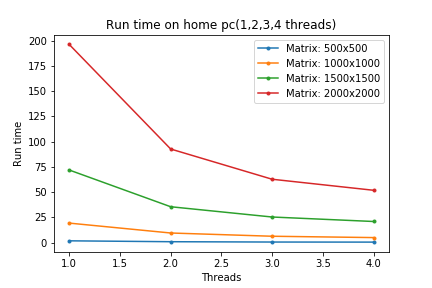
\includegraphics[scale=0.4]{pc/RuntimeMypc.png}~
		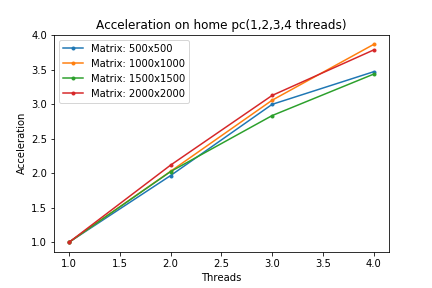
\includegraphics[scale=0.4]{pc/AccelerationMypc.png}
		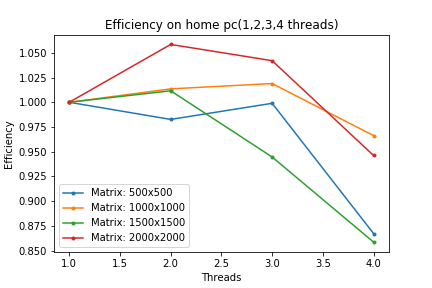
\includegraphics[scale=0.4]{pc/EfficiencyMypc.png}
		\caption{графики результатов работы на домашнем ПК}
		
		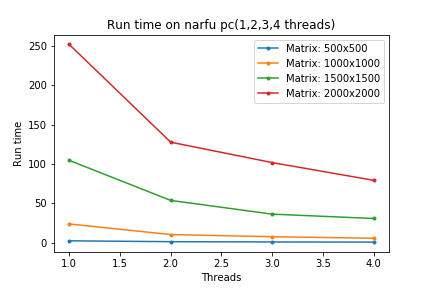
\includegraphics[scale=0.4]{narfupc/RuntimeNarfupc.png}~
		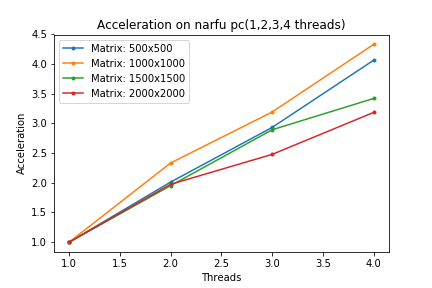
\includegraphics[scale=0.4]{narfupc/AccelerationNarfupc.png}
		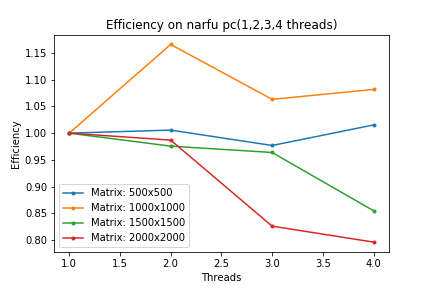
\includegraphics[scale=0.4]{narfupc/EfficiencyNarfupc.png}
		\caption{графики результатов работы ПК(ауд.301)}

	\end{figure}

	\begin{figure}
		\centering
		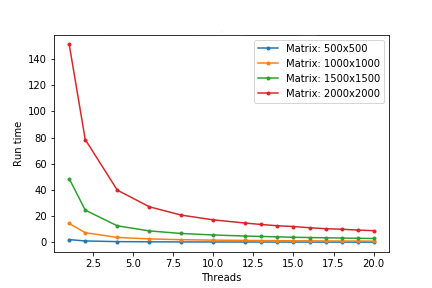
\includegraphics[scale=0.4]{cluster/RuntimeCluster.png}~
		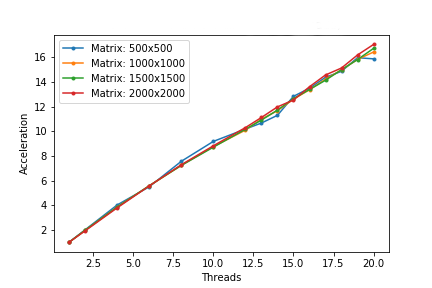
\includegraphics[scale=0.4]{cluster/AccelerationCluster.png}
		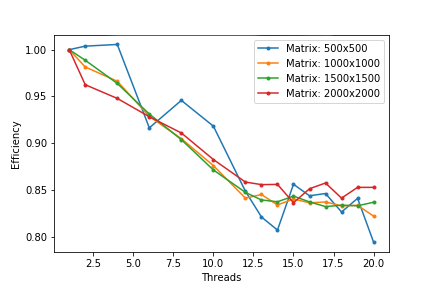
\includegraphics[scale=0.4]{cluster/EfficiencyCluster.png}
		\caption{графики результатов работы на кластере САФУ}
		
		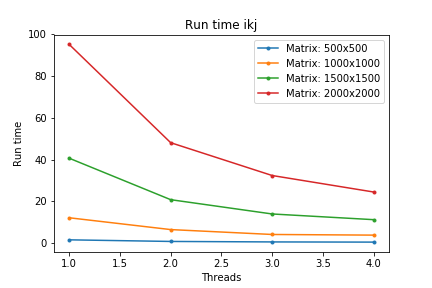
\includegraphics[scale=0.4]{ikj/ikj_Runtime.png}~
		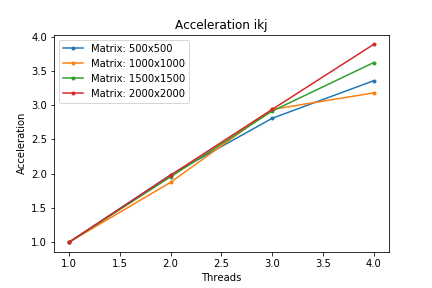
\includegraphics[scale=0.4]{ikj/ikj_Acceleration.png}
		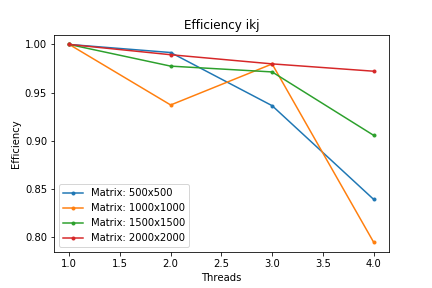
\includegraphics[scale=0.4]{ikj/ikj_Efficiency.png}
		\caption{графики результатов работы при смене переменных цикла на IKJ}
	\end{figure}
	
\newpage
\section{Вывод}
По рис. 1-3 можно сделать вывод, что параллельный алгоритм умножения матриц намного эффективнее и быстрее последовательного.
Также были замечены "скачки" в графиках эффективности. Данные "скачки" демонстрируют принцип работы кэша процессора. Когда мы выполняем расчеты, в кэш заносится не один информационный элемент, а сразу целый блок, что ускоряет работу программы. При изменении организации циклов наиболее быстро будет выполняться умножение матриц c организацией внутреннего цикла по переменной j (IKJ, KIJ). По моему мнению, так происходит из-за особенности выделения памяти (память выделяется по строкам, и обращение к следующему элементу строки гораздо быстрее, чем обращение к следующему элементу столбца). Таким образом, зная, как выделяется память в C++, можно ускорить работу своей программы.
\end{document}